\scanpage{10}
\deleted{Supposons \unsure{maintenant que} \(\varphi_f\) \illegible{1}}

On posera, pour une fonction mesurable \deleted{positive}
\[
(12)\qquad\Delta(f)=\Delta^{\unsure{-}}_{|f|}(|M|)=\uuline{\exp}\int_M\log|f|\,dm
\]
\deleted{\(\Delta\) existe \unsure{si}}\par\deleted{donc}
\(\Delta(f)\) existe \deleted{\(\unsure{\Psi_f}\) \unsure{existe}} si \(\log|f|\) est sommable sur l'ens des points où elle est positive. \(0\leq\Delta(f)<+\infty\).
\(\Delta\) jouit des propriétés d'un \inserted{module de} déterminant, en particulier
\[
(13)\qquad\Delta(fg)=\Delta(f)\Delta(g)\qquad\Delta(1)=1
\]
\figure{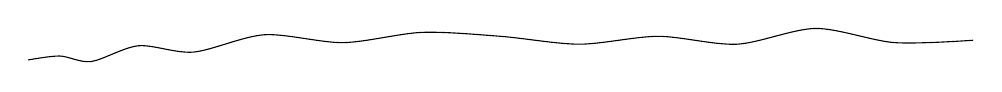
\begin{tikzpicture}[x=1cm,y=1cm]
\draw plot[smooth] coordinates {(0,0) (.4,.05) (.8,-.02) (1.4,.18) (2.1,.1) (3,.32) (4,.22) (5,.35) (6,.3) (7,.2) (8,.3) (9,.2) (10,.4) (11,.22) (12,.25)};
\end{tikzpicture}}

Supposons que \(|M|<+\infty\). On vérifie aussitôt que \deleted{\unsure{si} \(f\)}\inserted{pour une fonction mesurable positive sur \(M\), on a} \deleted{\unsure{étant son} réarrangement décroissant \(\varphi_f\), alors}\par\deleted{il en est de même}\par\deleted{\(\unsure{\varphi_{1+f}}\) \unsure{et}}
\[
(14)\qquad\varphi^-_{\unsure{\lambda|1}+f}(t)\unsure{=|\equiv}\unsure{\lambda|1}+\varphi_f^-(t)\qquad\text{si }\unsure{0<t|0\leq t}\leq|M|
\]
(si \(\varphi_f\) existe; si même \(|M|=\infty\), \(\varphi_{1+f}\) n'existe pas \inserted{\unsure{à priori}} si \(f\geq0\), \deleted{Cependant}\inserted{nous} \unsure{pouvons encore le définir} par (14). Alors \(\log\varphi_{1+f}(t)=\log(1+\varphi_f)\)\deleted{\unsure{si} \(\Phi_f\) existe, \unsure{alors}}\inserted{\(\log(1+\varphi_f)\)} qui est une fonction positive. Si on suppose que \(\Phi_f\) existe, alors \(\log(1+\varphi_f)\) est sommable au voisinage de \(0\) (et dans ce cas seulement). On pose, par définition
\[
(15)\qquad\Delta_{\unsure{\lambda|1}+f}(t)=\exp\int_0^t\log|1+\varphi_f(\unsure{s|u})|\,ds
\qquad0\leq|t|\leq|M|
\]
cette notation est cohérente avec (9) quand cette dernière a un sens, i.e. si \(|M|<+\infty\). On a d'ailleurs
\[
(16)\qquad\Delta_{1+f}(|M|)=\Delta(1+f)
\]
\figure{\begin{tikzpicture}[x=1cm,y=1cm]
\draw (0,.1)--(0,-.2);
\draw plot[smooth] coordinates {(0,.1) (.6,0) (1,.06) (1.8,-.15) (3,.12) (4,-.04) (5,.05) (6,-.1) (7,-.12) (8,.2) (9,.08) (10,.22) (11,.17) (12,.14)};
\draw (12,.14)--(12,1.3)--(11.7,1.3);
\end{tikzpicture}}

Soit \(\nu\) une mesure positive sur \(R_*\), telle que \(\int_a^\infty d\nu<+\infty\) pour tout \(a\) (\(a\) non nécessairement positif). \deleted{soit \(M\geq\|\nu\|\)}\inserted{Supposons \(\|\nu\|=+\infty\) (\unsure{ou} \(0\leq\|\nu\|\leq M<+\infty\)).} Alors il existe une fonction décroissante \(\varphi\) et une seule sur \deleted{\(\unsure{R_*}\)}\inserted{\(R_*^+\) (resp. \deleted{\(\unsure{]0,M[}\)} sur \(]0,M[\))} telle que \(\mu_\varphi=\unsure{\nu|\mu}\). Cette \(\varphi\) est positive si et seulement si \(\unsure{\mu|\nu}\) est portée par \(R_*^+\). \deleted{On} Soit maintenant \(f\) telle

\margin{\unsure{Le bon} \unsure{cas où} \(\|\nu\|<+\infty\) !\par\deleted{\unsure{dim.}}\par\unsure{on peut prendre} \illegible{1} \unsure{à l'infini}}

\mspage{11}
